% Auriga theme
% find the most up-to-date version here: https://github.com/anishathalye/auriga

\documentclass[14pt,aspectratio=169]{beamer}
\usepackage{pgfpages}
\usepackage{fancyvrb}
\usepackage{tikz}
\usepackage{pgfplots}
\usepackage{booktabs}
\pgfplotsset{compat=1.18}

% Use natbib with author-year citation style
%\usepackage[authoryear]{natbib}

% Add the bibliography style compatible with author-year
%\bibliographystyle{plainnat}

\setbeamertemplate{bibliography item}[text]

\renewcommand{\footnote}[1]{
    \begin{tikzpicture}[remember picture,overlay]
        \node[anchor=north east, xshift=-0.2cm, yshift=-0.2cm] at (current page.north east) {\footnotesize #1};
    \end{tikzpicture}
}
\usetheme{auriga}
\usecolortheme{auriga}
\setbeamercolor{math text}{fg=blue}

\newcommand\blfootnote[1]{%
\begingroup
\renewcommand\thefootnote{}\footnote{#1}%
\addtocounter{footnote}{-1}%
\endgroup
}

%\setbeamertemplate{footline}[]
%\renewcommand\footnotemark{}


% define some colors for a consistent theme across slides
\definecolor{red}{RGB}{181, 23, 0}
\definecolor{blue}{RGB}{0, 118, 186}
\definecolor{gray}{RGB}{146, 146, 146}
\title{Speculations \\ on \\ Test-Time Scaling}
\author{Sasha Rush \  Daniel Ritter}

\institute[shortinst]{Cornell}
% \institute[shortinst]{\inst{*} Preprint}

\setcounter{tocdepth}{1}
\begin{document}

\frame{\titlepage}

\begin{frame}{Outline}
	\tableofcontents
\end{frame}

\section{Introduction}

\begin{frame}[t]{}
	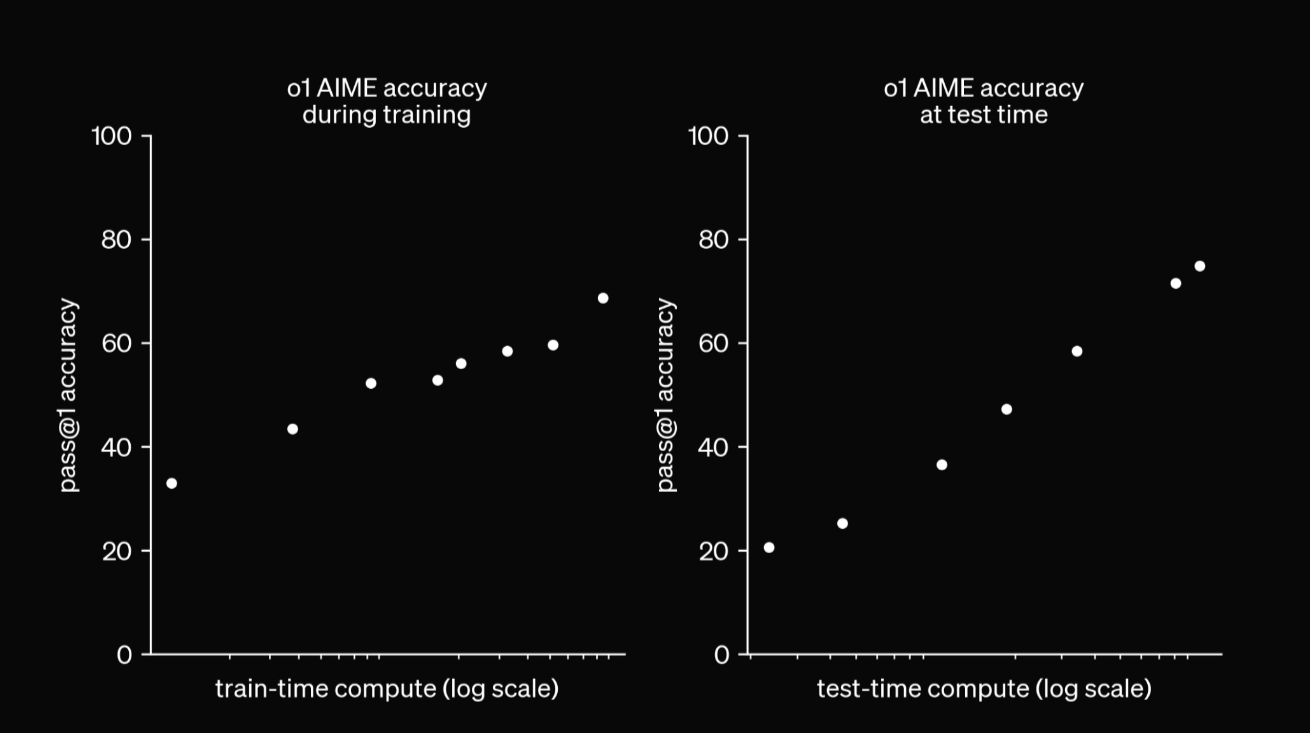
\includegraphics[width=\linewidth]{images/compute.png}
\end{frame}

\begin{frame}{Context}
	\begin{itemize}
		\item LLM (2018-2024) driven by training scaling
		\item Speculation: Benefit of static data running out
	\end{itemize}
	\blfootnote{}
\end{frame}

\begin{frame}{Implication}
	\begin{itemize}
		\item Breakthrough in large-scale RL Training
		\item
	\end{itemize}
	\blfootnote{}
\end{frame}

\begin{frame}{What have we seen?}
	\begin{itemize}
		\item Public demo model
		\item Strong result in constrained domains.
	\end{itemize}
	\blfootnote{}
\end{frame}

\begin{frame}{This Talk}
	\begin{itemize}
		\item Survey of the public literature
		\item Synthesis of discussions with expert
		\item Gossip and hearsay
	\end{itemize}
	\blfootnote{}
\end{frame}

\begin{frame}{Thanks}
	Lewis Tunstall, Edward Beeching, Aviral Kumar, Charlie Snell,
	Michael Hassid, Yoav Artzi, Risab Agarwal, Kanishk Gandhi,
	Wenting Zhao, Yuntian Deng, Nathan Lambert
\end{frame}

\section{The Clues}

\begin{frame}{What we know}
	Our large-scale \textbf{reinforcement learning algorithm} teaches the model
	how to think productively using its \textbf{chain of thought} in a highly
	\textbf{data-efficient} training process.
\end{frame}

\begin{frame}{What we know}
	\begin{itemize}
		\item RL - Signal from verifiable problems
		\item CoT - ``Thinking'' occurs in token stream
		\item Data Efficient - Fixed set of good problems
	\end{itemize}
\end{frame}

\begin{frame}{From Gossip}
	\begin{itemize}
		\item Single final model
		\item Not learned from expert examples
		\item
	\end{itemize}
\end{frame}

\begin{frame}{Chain of Thought}
	o1 learns to hone its chain of thought and refine the strategies it uses.
	It learns to recognize and \textbf{correct its mistakes}.
	It learns to \textbf{break down tricky steps} into simpler ones.
	It learns to try a \textbf{different approach} when the current one isn’t working.
\end{frame}

\begin{frame}{Review: Chain of Thought}
	\begin{itemize}
		\item
	\end{itemize}
	\blfootnote{}
\end{frame}

\begin{frame}{Planning}

\end{frame}

\begin{frame}{Backtracking}

\end{frame}

\begin{frame}{Strategies}

\end{frame}


\begin{frame}{Summary}
	\begin{itemize}
		\item Solves problems by very long CoT
		\item CoT includes ``thinking'' (search / planning)
		\item Core novelty: Inducing this behavior
	\end{itemize}
\end{frame}

\section{Notation}

\begin{frame}{Notation - Test-Time (No learning yet!)}
	\begin{itemize}
		\item $x$ - the problem specification
		\item $z \in {\mathcal{S}^T}$ - the chain of thought (CoT)
		\item $y \in {\mathcal Y}$ - the final answer
		\item $p(y | x) = \mathbb{E}_{z \sim p(z|x)} p(y|x,z)$ - model
	\end{itemize}
\end{frame}

\begin{frame}{Warm-up: Ancestral Sampling}
	\begin{columns}
		\begin{column}{0.5\linewidth}
			\begin{itemize}
				\item $\tilde{z} \sim p(z | x)$
				\item $\tilde{y} \sim p(y | x, z=\tilde{z})$
			\end{itemize}
		\end{column}
		\begin{column}{0.5\linewidth}
			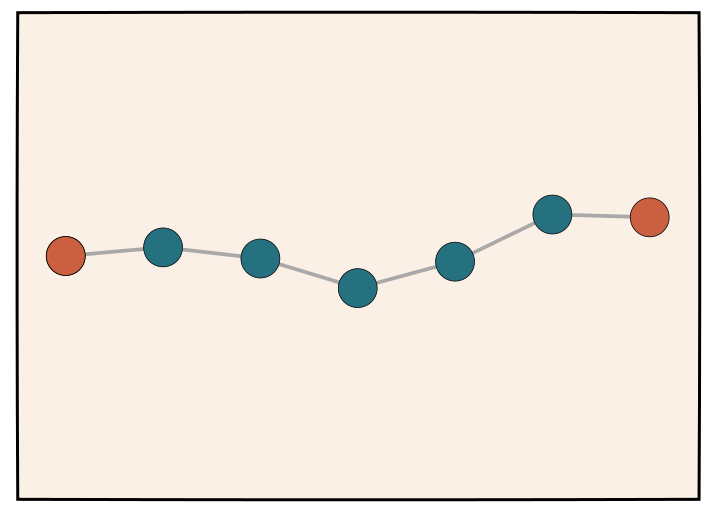
\includegraphics[width=\textwidth]{images/ancestral.png}
		\end{column}
	\end{columns}
    \vspace{1cm}
    $|\tilde{z}|$ is the amount of test-time compute
\end{frame}

\begin{frame}{Warm-up: Monte-Carlo (Self-Consistency)}
	\begin{columns}
		\begin{column}{0.5\linewidth}
			\begin{itemize}
				\item $\tilde{z} \sim p(z | x)$
				\item $\tilde{y} \sim p(y | x, \tilde{z})$
			\end{itemize}
            \vspace{1cm}
			Pick majority choice $\tilde{y}^i$
		\end{column}
		\begin{column}{0.5\linewidth}
			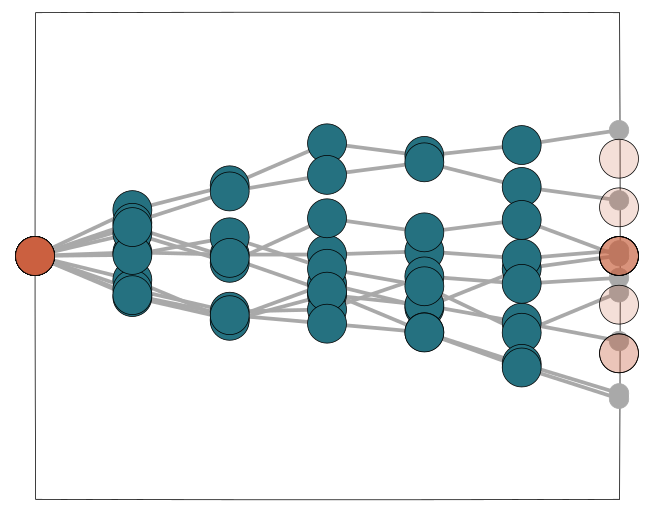
\includegraphics[width=\textwidth]{images/bwalk.png}
		\end{column}
	\end{columns}
\end{frame}

\begin{frame}{Notation - Verifier}
	\begin{itemize}
		\item $\text{Ver} : \mathcal{Y} \rightarrow \{0, 1\}$, tells us if an answer is correct or not
		\item Examples: Regular expression for math, unit test for code.
	\end{itemize}
\end{frame}


\begin{frame}{Warm up: Rejection Sampling / Best-of-N}
	\begin{columns}
		\begin{column}{0.5\linewidth}
			\begin{itemize}
				\item $\tilde{z} \sim p(z | x)$
				\item $\tilde{y} \sim p(y | x, \tilde{z})$
			\end{itemize}
		\end{column}
		\begin{column}{0.5\linewidth}
			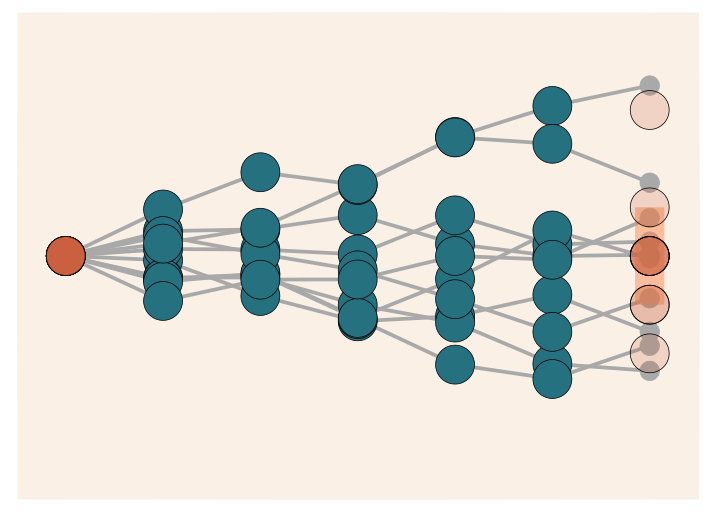
\includegraphics[width=\textwidth]{images/reject.png}
		\end{column}
	\end{columns}
    \vspace{1cm}
    We only keep the correct subset of $\tilde{y}$, $\{\tilde{y} : Ver(\tilde{y}) \}$\end{frame}

\begin{frame}{Variants:}
\end{frame}


\begin{frame}{Warm up: Monte-Carlo Roll-Outs}
	\begin{columns}
		\begin{column}{0.5\linewidth}
            \begin{itemize}
    			\item Given $x, z_{1:t}$ (a partial chain of thought) define expected reward as

    			$$\mathbb{E}_{y\sim p(y| z, x), z_{t:T} \sim p(z | z_{1:t}, x)}[Ver(y)]$$

    			\item Roll-outs apply MC to this expectation.
            \end{itemize}
		\end{column}
		\begin{column}{0.5\linewidth}
			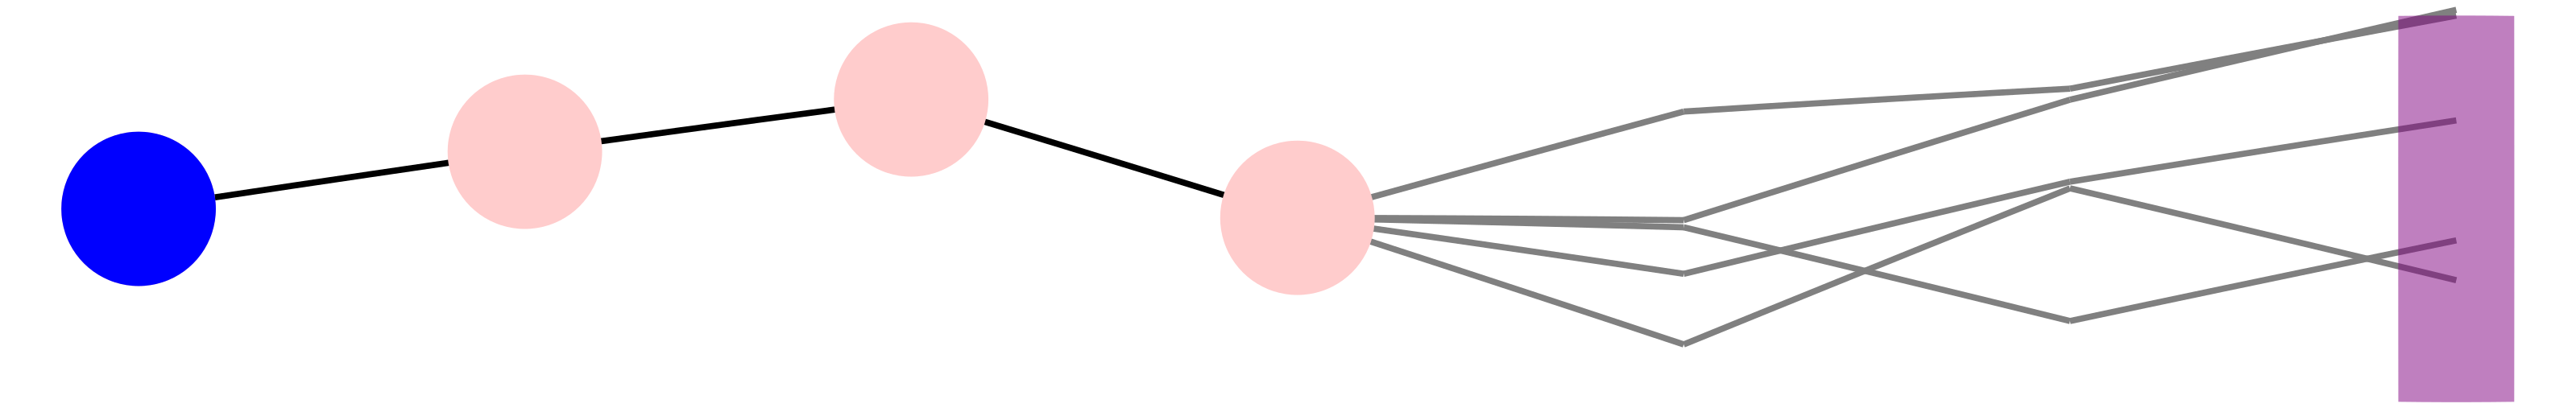
\includegraphics[width=\textwidth]{images/mcroll.png}
		\end{column}
	\end{columns}
\end{frame}



\begin{frame}{Goal: Learning}
	\begin{columns}
		\begin{column}{0.5\linewidth}
			\begin{itemize}
				\item $\max_{\theta} \sum \log p(y | x; \theta)$
				\item Intractable expectation over latent CoT
			\end{itemize}
		\end{column}
		\begin{column}{0.5\linewidth}
			%\includegraphics[width=\textwidth]{images/marginal.png}
		\end{column}
	\end{columns}
\end{frame}

\section{The Suspects}

\begin{frame}{Outline}
	\tableofcontents[hideallsubsections]
\end{frame}

\begin{frame}{The Suspects}
	\begin{itemize}
		\item Guess + Check
		\item Guided Search
		\item AlphaZero
		\item Learn to Search
		\item Wildcard
	\end{itemize}
\end{frame}

%\begin{frame}{A Note About Names}
%	\begin{itemize}
%		\item Many different communities
%		\item Names conflict and overlap with past methods
%		\item This talk: First explain, then discuss names
%	\end{itemize}
%\end{frame}


\subsection{Guess + Check}

\begin{frame}{Informal: Guess + Check}
	\begin{itemize}
		\item Sample $N$ CoTs
		\item Check if successful
		\item Train on good ones
	\end{itemize}
\end{frame}

\begin{frame}{Formalization: Rejection Sampling EM}
	$$\max_{\theta} \sum \log p(y | x; \theta) = \sum \log E_{z} p(y, z | x)$$
	\begin{itemize}
		\item E-Step: Sample $\tilde{z}$ from the posterior with Rejection Sampling
		\[ \tilde{z} \sim p(z | \text{Ver}(y)=1, x) \]
		\item M-Step: Fit $\theta' \gets \arg\max_{\theta}
			      \sum_{z\in \mathcal{Z}} \log p(z | x;\theta)$
	\end{itemize}
\end{frame}



\begin{frame}{Terminology}
    \blfootnote{\cite{Zelikman2022-id,Gulcehre2023-vk,Singh2023-eb}}
	\begin{itemize}
		\item STaR
		\item ReST
		\item ReST-EM
		\item Filtered Rejection Sampling
		\item Best-of-N Training
	\end{itemize}
\end{frame}


\begin{frame}{Batched }
	\begin{itemize}
		\item Batched -> Compute trajectories first, then train with behavioral cloning
		\item Online -> Use policy gradient-like steps to update after each example
	\end{itemize}
\end{frame}


%\begin{frame}{Offline}
%	\begin{itemize}
%		\item Batch servers to sample
%		\item Check if successful
%		\item Train on good ones
%	\end{itemize}
%\end{frame}


%\begin{frame}{Online}
%	\begin{itemize}
%		\item Sample N CoTs
%		\item Check if successful
%		\item Train on good ones
%	\end{itemize}
%\end{frame}

\begin{frame}{Empirical Results}

	Find a good chart from a paper.
	Best representative.

	Improvement over self-consistency. ([Daniel] Surprisingly almost no direct comparison to self-consistency in a lot of what we've looked at, RestEM mentions majority voting, and says they improve on it by 4 percent but it's not in any of the figures, still looking for a good picture here).
\end{frame}



\begin{frame}{Why might this be right?}
	\begin{columns}
		\begin{column}{0.5\linewidth}
			\begin{itemize}
				\item Extremely simple and scalable
				\item Good baseline in past work
			\end{itemize}
		\end{column}
		\begin{column}{0.5\linewidth}
			\begin{itemize}
				\item No evidence this learns to correct, plan
				\item Well-explored in literature with marginal gains
			\end{itemize}
		\end{column}
	\end{columns}
\end{frame}

\begin{frame}{Deeper}
	\begin{itemize}
		\item Rejection sampling may be really inefficient.
		\item Particularly on hard problems, may get no signal
	\end{itemize}
\end{frame}

\subsection{Guided Search}

\begin{frame}{Informal: Guided Search}
	\begin{itemize}
		\item During CoT sampling, use a ``guide'' to
		      correct trajectories
		\item Check if final versions are successful
		\item Train on good ones
	\end{itemize}
\end{frame}


\begin{frame}{Beam Search with Guide}
	\begin{columns}
		\begin{column}{0.5\linewidth}
			\begin{itemize}
                \item $r: S^T \rightarrow \mathbb{R}$ is the guide/reward function
				\item $\tilde{z_{t}} \sim p(z_{t} | x, z_{1:t-1})$
				\item $\tilde{y} \sim p(y | x, \tilde{z})$
			\end{itemize}
		\end{column}
		\begin{column}{0.5\linewidth}
			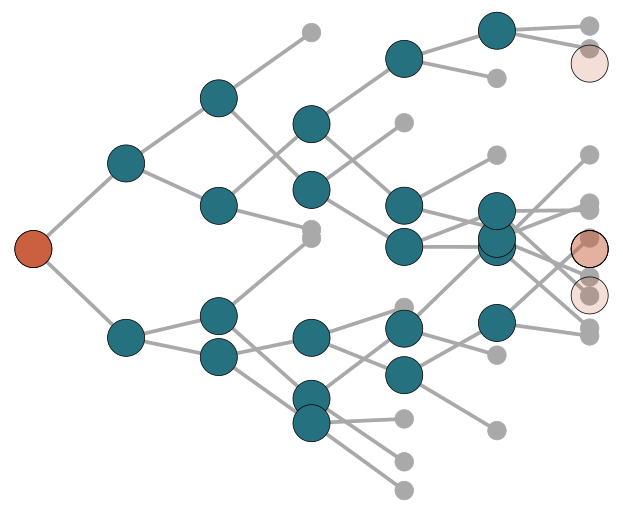
\includegraphics[width=\textwidth]{images/beam.png}
		\end{column}
	\end{columns}
\end{frame}


\begin{frame}{What to use as Guide?}
	\begin{itemize}
		\item Roll-outs
		\item Learned Reward Model
	\end{itemize}
\end{frame}


\begin{frame}{Beam Search with Roll-Outs}
	\begin{columns}
		\begin{column}{0.5\linewidth}
			Beam Roll
		\end{column}
		\begin{column}{0.5\linewidth}
			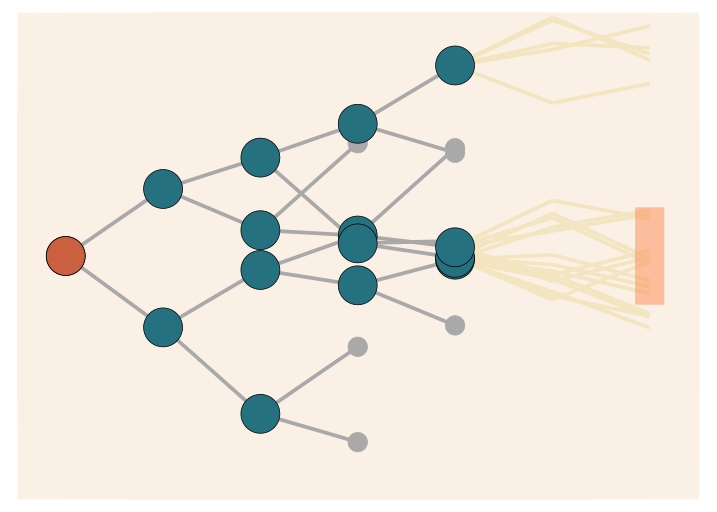
\includegraphics[width=\textwidth]{images/beamroll.png}
		\end{column}
	\end{columns}
\end{frame}


\begin{frame}{Amortized Roll-Outs}
	\begin{columns}
		\begin{column}{0.5\linewidth}
			Given $x, z_{1:t}$ define expected reward as

			$\mathbb{E}_{y\sim p(y| z, x), z_{t:T} \sim p(z | z_{1:t}, x)}[Ver(y)]$

			Roll-outs apply MC to this expectation.
		\end{column}
		\begin{column}{0.5\linewidth}
			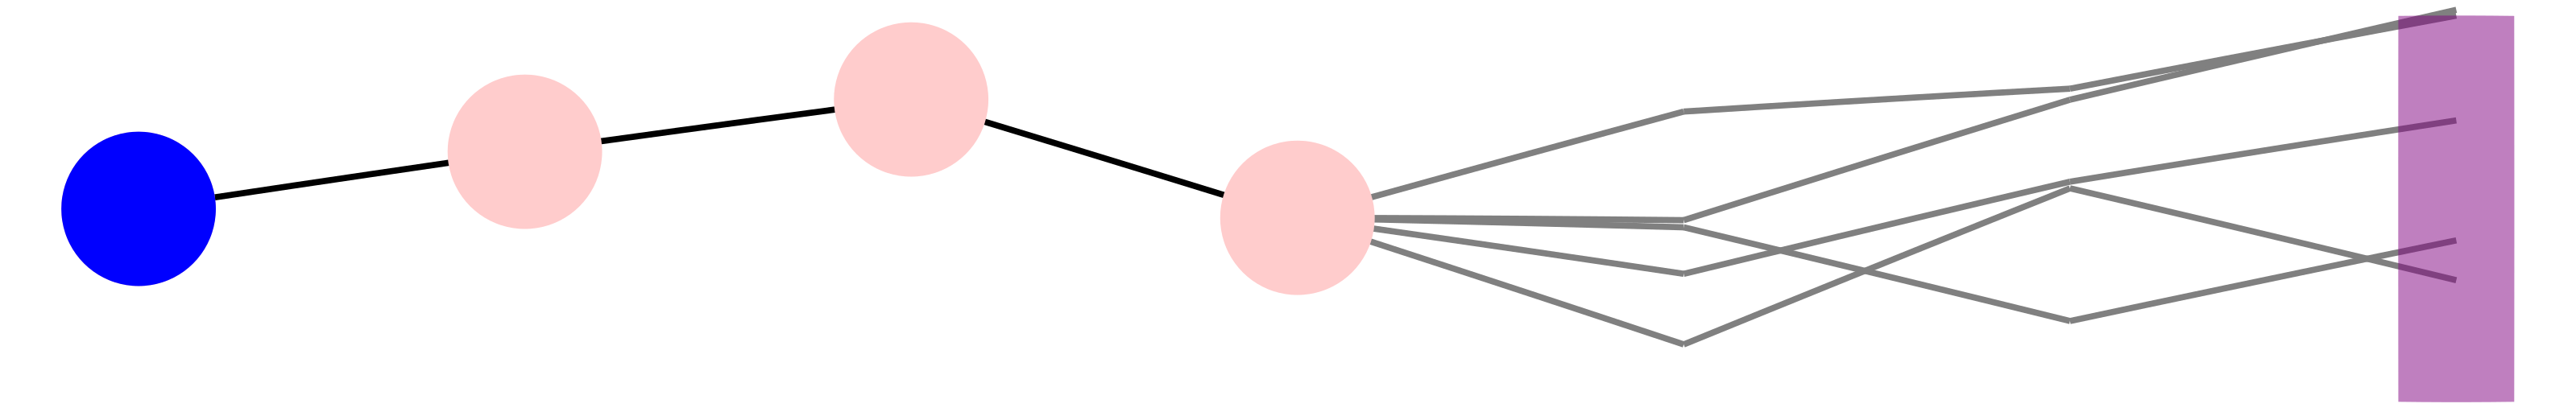
\includegraphics[width=\textwidth]{images/mcroll.png}
		\end{column}
	\end{columns}
\end{frame}

\begin{frame}{What about test time?}
	\begin{itemize}
		\item Learned rewards can improve test-time without verifier.
		\item
	\end{itemize}
\end{frame}


\begin{frame}{Terminology}
	\begin{itemize}
		\item Value
		\item PRM
		\item PAV
		\item Math Shepard.
		\item snell.
	\end{itemize}
	\blfootnote{\cite{Uesato2022-aw}}
\end{frame}


\begin{frame}{Why might this be right?}
	\begin{itemize}
		\item OpenAI is exploring
		\item Makes RS more efficient.
		\item Learned rewards are effective
	\end{itemize}
	\begin{itemize}
		\item Assumption: o1 is a single test-time model
		      (although could train or distill-in)
		\item Not clear if it learns planning.
	\end{itemize}
\end{frame}


\begin{frame}{Deeper}
	\begin{itemize}
		\item Improving search seems critical.
	\end{itemize}
\end{frame}

\subsection{AlphaZero / MuZero}

\begin{frame}{Reminder: AlphaZero}
	Picture
\end{frame}

\begin{frame}{Informal: AlphaZero}
	\begin{itemize}
		\item Guided-search with exploration
		\item Collect the best CoT
		\item Train on good ones, repeat
	\end{itemize}
\end{frame}

\begin{frame}{Formalized: Expert Iteration}
	\begin{itemize}
		\item Iterative algorithm combining learned model + expert search.
		\item Each iteration, search algorithm factors in learned confidence.
	\end{itemize}
	\blfootnote{\cite{Anthony2017-dm}}
\end{frame}

\begin{frame}{UCB for exploration}
	\begin{itemize}
		\item
	\end{itemize}
\end{frame}


\begin{frame}{Empirical Results}

	Find a good chart from a paper.
	Best representative.

	Improvement over STarish.
\end{frame}


\begin{frame}{Why might this be right?}
	\begin{itemize}
		\item Major demonstrated RL result
		\item
	\end{itemize}
	\begin{itemize}
		\item
		\item
	\end{itemize}
\end{frame}


\begin{frame}{Deeper}
	\begin{itemize}
		\item Can we force the model to search?
	\end{itemize}
\end{frame}

\subsection{Learning to Correct}

\begin{frame}{Informal: Learning to Correct}
	\begin{itemize}
		\item Sample $N$ Successful CoTs
		\item Edit $z\rightarrow z'$ to inject incorrect expansions before
		      correct ones.
		\item Train on $z'$ trajectories
	\end{itemize}
\end{frame}

\begin{frame}{Formalized: Stream of Search}
	\begin{itemize}
		\item
		\item
	\end{itemize}
	\blfootnote{\cite{Gandhi2024-vs}}
\end{frame}


\begin{frame}{Empirical Results}
	Score results
\end{frame}


\begin{frame}{Why might this be right?}
	\begin{itemize}
		\item
		\item
	\end{itemize}
\end{frame}

\begin{frame}{Why might this be wrong?}
	\begin{itemize}
		\item
		\item
	\end{itemize}
\end{frame}

\section{No Verifier}

\begin{frame}{No verifier}
	\begin{itemize}
		\item
	\end{itemize}
	\blfootnote{\cite{Brown2024-bs}}
\end{frame}



\section{Conclusions}

\begin{frame}{}
\end{frame}

\begin{frame}[allowframebreaks]{Reference}
	\bibliographystyle{apalike}
	\bibliography{../o1.bib,../o1.extra.bib}
\end{frame}

\end{document}
